 \section{非线性规划}
 \subsection{非线性规划问题及其数学模型}
非线性规划 (non-linear programming) 问题不要求目标函数、约束条件都为线性形式,较之线性规划问题以及由其发展出来的整数规划、目标规划,
非线性规划的应用更加广泛,一般的线性规划仅仅是非线性规划的特例而已。由于约束条件的放宽,非线性规划问题可以
更接近于现实生活中的种种问题,同时,求解难度也提高了很多。用矩阵和向量来表示非线性函数的数学模型如下:
 \begin{equation}\label{eq:nlp}
\begin{array}{l}
 \min \ z=f({\mathbf{x}})  \\
 \text{s.t.}\left\{ \begin{array}{ccccc}
   \mathbf{x_l}& \leqslant&    \mathbf{x}  & \leqslant  & \mathbf{x_u} \\
   \mathbf{b_l}& \leqslant&   \mathbf{Ax}  & \leqslant  & \mathbf{b_u} \\
   \mathbf{c_l}& \leqslant&  \mathbf{c(x)} & \leqslant  & \mathbf{c_u}\\
 \end{array} \right.
 \end{array}
\end{equation}

模型 (\ref{eq:nlp}) 中,$z=f(\mathbf{x})$ 为目标函数,三个约束条件中,第一个为定义域约束,第二个为线性约束 ($\mathbf{A}$ 为系数矩阵),
第三个为非线性约束\footnote{注意:$\mathbf{c(x)}$ 为一组非线性约束函数,而不局限于一个。}。当目标函数和
约束函数光滑时,称之为光滑的非线性规划,其求解的难度要小于非光滑的非线性规划。
\subsection{用 \pkg{Rdonlp2} 包求解光滑的非线性规划}
对于无约束或者约束条件相对简单的非线性优化问题,\pkg{stats} 包中的 \fun{optim()}、\fun{optimize()}、 
 \fun{constrOptim()}、\fun{nlm()}、\fun{nlminb()} 等函数可以完美地解决,并且它们的使用方法相当简单。
 鉴于该包为默认安装包,大多数人比较熟悉,下面着重探讨专门解决非线性优化的 \pkg{Rdonlp2} 包\citep{Rdonlp207}
 的用法。


\R 中,\pkg{Rdonlp2} 包是一个非常强大的包,可以方便快速地解决光滑的非线性规划问题。该包在学习、研究中可以自由
使用,其它用途则需要授权。核心函数为 \fun{donlp2()},可以求连续非线性函数的最值 (默认求最小值) ,用法如下:

\begin{verbatim}
 donlp2(par, fn,
        par.upper=rep(+Inf, length(par)),
        par.lower=rep(-Inf, length(par)),

        A = NULL,
        lin.upper=rep(+Inf, length(par)),
        lin.lower=rep(-Inf, length(par)),

        nlin = list(),
        nlin.upper=rep(+Inf, length(nlin)),
        nlin.lower=rep(-Inf, length(nlin)),

        control=donlp2.control(),
        control.fun=function(lst){return(TRUE)},
        env=.GlobalEnv,
        name="Rdonlp2")
\end{verbatim}

该函数的参数较多,下面分类对它们进行详细解释:
\begin{enumerate}
\item 初始值、目标函数及自变量定义域:
\begin{description}
\item [par] 向量,迭代初始值。
\item [fn] 连续型函数,函数自变量限制为 1 个 (自变量一般为向量,这样可以包含多个参数),函数的返回值
                 为优化目标。
\item [par.upper 和 par.lower] 向量,分别为自变量的上下界限,即模型 (\ref{eq:nlp}) 中的
                 $\mathbf{x_u}$ 和 $\mathbf{x_l}$,它们的长度应该和向量 \rcode{par} 
                相等。如果变量无界,必须用正无穷 (+Inf) 和负无穷大 (-Inf) 来表示。可以看出,自变量默认
                无界,可以取全体实数。
\end{description}

\item 线性约束:
\begin{description}
\item [A]线性约束矩阵,即模型 (\ref{eq:nlp}) 中的矩阵 $\mathbf{A}$,其列的长度必须和向量 \rcode{par} 相等 (即总变量个数),
            其行的长度必须和线性约束的个数相等。
\item [lin.upper 和 lin.lower]向量,分别为线性约束条件的上下界限,即模型 (\ref{eq:nlp}) 中的
                 $\mathbf{b_u}$ 和 $\mathbf{b_l}$,它们的长度应该和线性约束的个数相等。
                如果某个线性约束无界,必须用正无
                穷 (+Inf) 
                或负无穷大 (-Inf) 来表示。如果某一个线性约束取固定值,那么只要设置它在 \rcode{lin.upper} 和
                 \rcode{lin.lower} 两个向量中对应
                位置都为该固定值即可 (如 $ax_1+bx_2=k$,可化为 $k\leqslant ax_1+bx_2 \leqslant k$,即上下界都为 k),
                这方法同样适合于下面要说的非线性约束条件的控制。
\end{description}
\item 非线性约束:
\begin{description}
\item [lin]列表,其中的元素为表示非线性约束条件的函数。
\item [nlin.upper 和 nlin.lower]向量,分别为非线性约束条件的上下界限,即模型 (\ref{eq:nlp}) 中的
                 $\mathbf{c_u}$ 和 $\mathbf{c_l}$,它们的长度应该和非线性约束的个数相等。
                如果某个非线性约束无界,必须用正无穷 (+Inf) 
                或负无穷大 (-Inf) 来表示。
\end{description}

\item 控制参数:
\begin{description}
\item[control]     控制参数,为 donlp2.control(),可以修改一些关于算法的参数和输出参数,可以根据实际要求修改。
\item[control.fun] 控制函数。
\item[env]  运行环境,一般不需要更改。
\item[name] 字符变量,如果不是默认值,则会在程序运行时在工作目录生成两个以 \rcode{name} 为主文件名,
            后缀分别为 pro、mes 的文件,其中 name.pro 文件为优化问题运行结果,name.mes 文件为警告及其它信息。
\end{description}
\end{enumerate}
 \begin{exmp}
求下列有约束的非线性规划问题。
\begin{equation*}
\begin{array}{l}
 \min \ z=x^2\sin y  + y^2\cos x  \\
 s.t.\left\{ \begin{array}{l}
  - 100 < x < 100 \\
  - 100 < y < 100 \\
  1\leqslant 3x - y   \leqslant 3\\
  x  + y   \geqslant 2\\
  \sin x\cos y \leqslant 0.6\\
  xy = 2
 \end{array} \right.
 \end{array}
\end{equation*}
 \end{exmp}
\noindent{{\textbf  解:}这是一个非线性规划问题。R 代码如下:}
\begin{Verbatim}
library(Rdonlp2)                          #载入包
p = c(10,10)                              #迭代初始值
par.l= c(-100,-100); par.u = c(100,100)   #自变量定义域约束
fn = function(x){
  x[1]^2*sin(x[2])+x[2]^2*cos(x[1])
}                                         #目标函数
A = matrix(c(1,1,3,-1),2,byrow=TRUE)
lin.l = c(2,1);lin.u = c(+Inf,3)          #7-8行构成线性约束
nlcon1 = function(x){
  x[1]*x[2]
}
nlcon2 = function(x){
  sin(x[1])*cos(x[2])
}
nlin.l = c(2,-Inf)
nlin.u = c(2,0.6)                          #9-16行构成非线性约束
ret = donlp2(p, fn, par.u=par.u, par.l=par.l,A,lin.l=lin.l,lin.u=lin.u,
             nlin=list(nlcon1,nlcon2), nlin.u=nlin.u, nlin.l=nlin.l)
\end{Verbatim}

运行程序,从输出结果\footnote{输出结果很多,有关于运行时间的,有关于中间过程的,也有关于算法参数的,在此
仅列出最感兴趣的输出。}中可以找到下面结果:
\begin{Verbatim}
 KT-conditions satisfied, no further correction computed
 optimal value of f =   2.28705347564892e+00
 optimal solution x =
  1.40307592849219e+00  1.42543960692795e+00
\end{Verbatim}

其中第 1 行表示求解成功,第 2 行表示此时目标函数最小值为 2.287(保留三位小数,后面也是如此),3 - 4 行
表示 x,y 分别为 1.403,1.425。


下面利用该包求解 Rastrigin 函数的最小值,由于该函数族极值点很多,而最值点仅有一个,
因而被广泛运用于测试各类优化算法,先选择一个二元的 Rastrigin 函数:
\[
 \min \ f(X) = \sum\limits_{i = 1}^2 {(x_i^2  - 10\cos (2\pi x_i ) + 10)}
\]

首先画出该函数在 x,y 区间都为 $[-5,5]$ 时的三维曲面图和颜色图,程序如下:
\begin{Verbatim}
a = 5
x = seq(-a, a, 0.01)
y = seq(-a, a, 0.01)
f = function(x, y){
    x^2 - 10*cos(2*pi*x) + y^2 - 10*cos(2*pi*y) + 20
}
z = outer(x, y, f)
image(x,y,z, col=heat.colors(24))      #画颜色图
library(rgl)                           #该包可以画出漂亮的三维曲面图
zorder = rank(z)
persp3d(x, y, z, col = rainbow(as.integer(max(zorder)))[zorder])
\end{Verbatim}
\begin{figure}
\begin{minipage}[t]{0.50\linewidth}
\centering
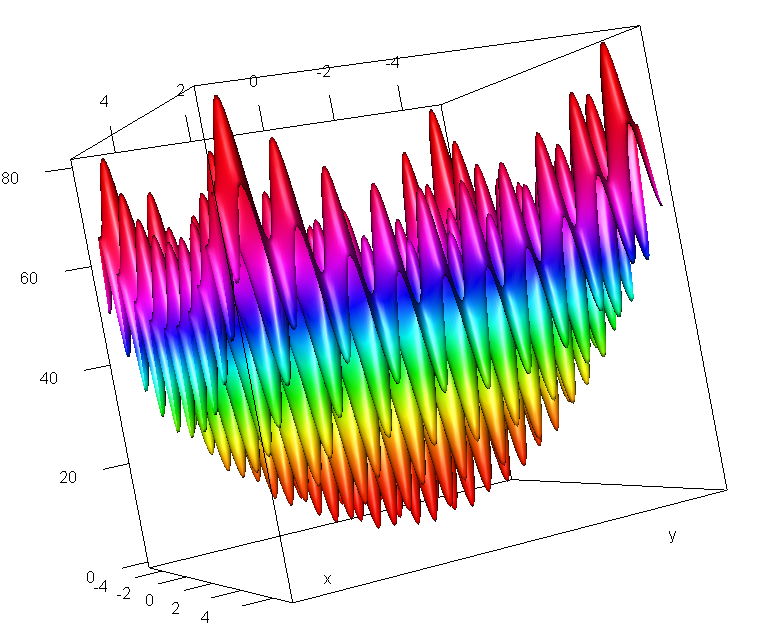
\includegraphics[width=\textwidth]{./pic/dim3.png}
\caption{三维曲面图 \label{fig:sanwei}}
\end{minipage}
\hfill
\begin{minipage}[t]{0.50\linewidth}
\centering
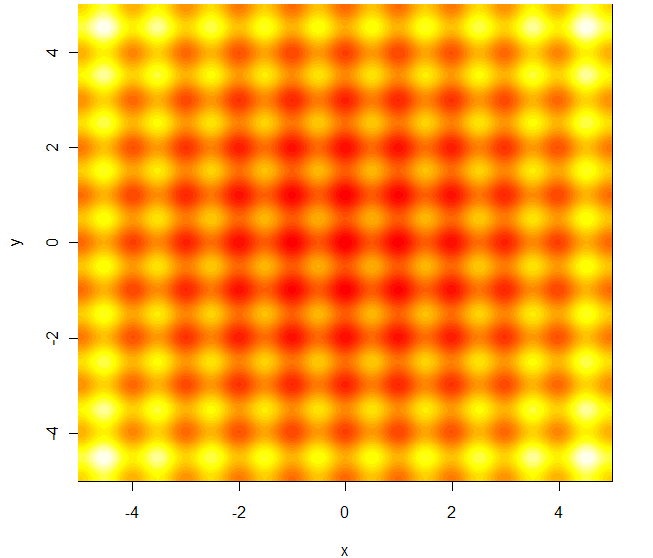
\includegraphics[width=\textwidth]{./pic/a.png}
\caption{颜色图\label{fig:color}}
\end{minipage}
\end{figure}

图 \ref{fig:sanwei} 为 Rastrigin 函数的三维曲面图,从图中可以看出,曲面图在该区域内
 (这里才仅仅取了很小的区域!) 有很多“尖刺”,这些“尖刺”就是极值点。
图 \ref{fig:color} 为 Rastrigin 函数的颜色图,函数值越小,颜色越深。红色点 (即深色点) 
即为局部极小点,可以看出仅仅在该区域内,函数已经有 121 个极小点了,这就使得 Rastrigin 函数最小点的求解变
得非常困难。现在用 \pkg{Rdonlp2} 包来求该函数的最小点。\\
{\textbf  解:}R 代码和部分运行结果如下:
\begin{Verbatim}
> library(Rdonlp2)
> fn=function(x){
>   f=sum(x^2-10*cos(2*pi*x)+10)  ##Rastrigin函数,参数x为向量,长度不定
> }
> par=c(-500,+500)                ##随便定义一个偏离最优解较远的初时迭代向量
> ret=donlp2(par,fn)
 optimal value of f =   0.00000000000000e+00

 optimal solution  x =
  3.31453975377372e-10 -3.31453975377372e-10
\end{Verbatim}

运行程序,可以发现最优解成功找到,目标函数最小值为 0(此时$x=0$,$y=0$),所耗时间极短。可以看出,\pkg{Rdonlp2} 
包处理该优化问题游刃有余,现在增加难度,求解有 1000 个变量的 Rastrigin 函数的最小值:
\[
 \min \ f(X) = \sum\limits_{i = 1}^{1000} {(x_i^2  - 10\cos (2\pi x_i ) + 10)}
\]

在 1000 维空间中,该函数的极小点奇多无比,求解非常困难。程序代码如下:
\begin{Verbatim}
library(Rdonlp2)
fn=function(x){                 ##Rastrigin函数,参数x为向量,动态长度
  f=sum(x^2-10*cos(2*pi*x)+10)
}
par=rep(-500,1000)              ##初时迭代向值,长度为1000
ret=donlp2(par,fn)
\end{Verbatim}

观察程序,发现和上一个程序的区别仅仅是 \rcode{par} 参数不同,而 Rastrigin 函数完全一样,这是因为 \R 语言
相当灵活,Rastrigin 函数的参数 \rcode{x} 的长度为动态的,可以根据具体情况变动,非常方便。在
 CPU 为 1.70 Hz,内存为 512 M 的计算机上运行程序,17 秒后,得到正确结果 (目标函数最小值为 0,自变量全为 0,在此
省略输出结果),
由此可见该函数在解决非线性规划问题中的强大之处。必须要说的是,本文仅仅介绍了该包最基本的用法,详细的介绍参见相关的
帮助文档\footnote{详细的帮助文件见\url{http://arumat.net/Rdonlp2/}}。
%而 LINGO 在处理非线性规划上没有什么优势,
%得出的解一般也比较差。



\subsection{一般的非线性规划}
有些非线性优化问题很难通过常规算法求解,此时启发式算法是一个不错的选择。遗传算法、粒子群算法、模拟退火算法、蚁群
算法都属于典型的启发式算法,这里主要介绍遗传算法在最优化问题中的应用。遗传算法是一类可用于复杂系统优化
的搜索算法,与传统的优化算法相比,主要有以下特点:
\begin{itemize}
\item  遗传算法以决策变量的编码作为运算对象,不依赖于问题的具体领域,对问题的种类有很强的稳健性 (robustness)。
\item  遗传算法只需要影响搜索方向的目标函数和相应的适应度函数,无需导数、梯度等其它辅助信息。
\item  遗传算法使用多个点的搜索信息,具有隐含并行性。
\item  遗传算法使用概率搜索技术,而非确定性规则。
\end{itemize}

由于遗传算法的以上特点,遗传算法在函数优化、组合优化、生产调度、自动控制、机器人学、图象处理、人工生命、遗传编码和机器学
习等方面获得了广泛的运用,而遗传算法本身也出现了许多变种。


\R 中提供了关于遗传算法和最优化的若干个包,常见的有 \pkg{gafit}、\pkg{rgenoud}、\pkg{genalg} 等,需要说明的是遗传
算法属于大类算法,并不专门针对某一具体问题,因此任何包也不能涵盖了遗传算法所有内容。鉴于 \pkg{gafit} 包使用简
单、求解速度快,下面主要介绍 \pkg{gafit} 包\citep{gafit02}在最优化问题中的应用。\pkg{gafit} 包中
仅有一个同名函数 \fun{gafit()},其用法如下:

\begin{verbatim}
gafit(target, start, thermal=0.1, maxiter=50, samples=10, step=1e-3)
\end{verbatim}

其中,\rcode{target} 为目标函数 (求其最小值),其格式为表达式 (expression),该函数可以随心所欲,没有光滑的
限制。我们可以设置定义域、各种约束之外的函数值为正无穷大,这样就可以将所有光滑的、非光滑的、甚至怪异的约束
条件加进去,这充分体现了遗传算法的广泛适用性。
\rcode{start} 为初时迭代值,格式为列表,同时也确定了目标函数中变量的多少 (这是因为目标函数的参数经常为向量,长度
是浮动的),明确这一点非常重要。
\rcode{maxiter} 为最大迭代次数,默认值为 50。若需要较高的精度,可以将其调大。其余参数参见帮助文档。

%下面来看一个特殊的非线性规划问题,该问题中包含复数。
\begin{exmp}
首先解决一个光滑的非线性优化问题,测试函数为五元的 Rastrigin 函数。
\end{exmp}

\noindent{{\textbf  解:}\R 代码及运行结果如下:}
\begin{Verbatim}
> library(gafit)
> fn=function(x){                 ##参数x为向量,长度不定
+   f=sum(x^2-10*cos(2*pi*x)+10)
+ }
> ff=expression(fn(x))
> gafit(ff,list(x=rep(500,5)),maxiter=1000)
$x
[1]  1.310361e-10 -1.404543e-09 -9.206026e-10  1.058998e-09 -1.083024e-09

attr(,"score")
[1] 0
\end{Verbatim}

从运行结果可以看出,\fun{gafit()} 函数成功求得最优解。需要说明的是,由于遗传算法本身的特点,每次所求的解都不会相同,
当问题比较复杂时,相差也许很大,建议多次运行,再从中选取最优解。当用 \fun{gafit()} 来求变量更多的 Rastrigin 函数的最
小值时,发现很难得到合理的答案,这是由于 Rastrigin 函数局部极值过多的原因。


\begin{exmp}下面再解决更为一般的非线性优化问题,其目标函数为非连续的四元函数:
\[
\begin{array}{l}
\min \ z=\sum\limits_{i=1}^4 -|(1-x_i)x_i\sin (10\pi x_i)| \qquad 0\leqslant x \leqslant 1
 \end{array}
\]
\end{exmp}

\noindent{{\textbf  解:}\R 代码及运行结果如下:}
\begin{Verbatim}
> f = function(x){
+   if(all(0<x)&all(x<1))            ##限定定义域
+   y = sum(-abs((1-x)*x^2*sin(10*pi*x)))
+   else
+   y = Inf
+   y
+ }
> gafit(expression(f(x)), thermal = 0.005, samples = 100,
+       list(x = rep(0.2,4)), maxiter = 500)
$x
[1] 0.6502202 0.6502213 0.6502201 0.6502189

attr(,"score")
[1] -0.5915143
\end{Verbatim}

结果中,\verb|$x| 中的向量为所得的解,\verb|attr(,"score")| 为此时对应的函数值,这和理论值极为接近,
说明该函数得出了比较满意的解。
最后需要说明的是,该函数在解决变量少、连续函数的优化问题时,不如前面的各种方法,只有在目标函数和约束函数非光
滑且非常复杂的情况下,它的相对优势才能更好的体现出来。
